\documentclass{../../templates/lkx_pset}

\usepackage[T1]{fontenc}
\RequirePackage{mlmodern}

\title{Math 230a Problem Set 10}
\author{Lev Kruglyak}
\due{November 20, 2024}

\collaborator{AJ LaMotta}
\collaborator{Ignasi Vicente}

\renewcommand{\O}{{\operatorname{O}}}
\renewcommand{\GL}{\operatorname{GL}}
\providecommand{\Det}{\operatorname{Det}}
\providecommand{\T}{\mathbb{T}}
\providecommand{\HH}{\mathbb{H}}
\providecommand{\gfr}{\mathfrak{g}}
\providecommand{\SO}{\operatorname{SO}}
\providecommand{\SU}{\operatorname{SU}}
\providecommand{\su}{\mathfrak{su}}
\renewcommand{\sl}{\mathfrak{sl}}
\providecommand{\Spin}{\operatorname{Spin}}
\providecommand{\Sp}{\operatorname{Sp}}
\providecommand{\scB}{\mathscr{B}}
\providecommand{\op}[1]{\operatorname{#1}}

     \usepackage[mathscr]{euscript}

\providecommand{\calB}{\mathcal{B}}

\providecommand{\Aff}{\operatorname{Aff}}
\providecommand{\HH}{\operatorname{H}}

\providecommand{\longto}{\;\xrightarrow{\phantom{xxx}}\;}
\providecommand{\longisom}{\;\xrightarrow{\phantom{xx}\sim\phantom{xx}}\;}
\providecommand{\longsurj}{\;\xtwoheadrightarrow{\phantom{xxx}}\;}

\providecommand{\definefunction}[5]{
	\begin{array}{rcl}
		#1 : #2 & \xrightarrow{\phantom{---}} & #3 \\
		#4      & \xmapsto{\phantom{---}}     & #5
	\end{array}
}

\providecommand{\qtq}[1]{\quad\textrm{#1}\quad}

\usepackage{adjustbox}
\newcommand{\alt}{\mathord{\adjustbox{valign=B,totalheight=.6\baselineskip}{$\bigwedge$}}}

\providecommand{\Hdr}{\operatorname{H}_{\operatorname{dR}}}

\providecommand{\pp}[2]{\frac{\partial #1}{\partial #2}}
\providecommand{\pps}[1]{\partial/\partial #1}


\ExplSyntaxOn
\NewDocumentCommand{\lkxto}{ O{} }{%
	\mathrel{\;\xrightarrow{\hphantom{xx}#1\hphantom{xx}}\;}
}
\NewDocumentCommand{\lkxmapsto}{ O{} }{%
	\mathrel{\;\xmapsto{\hphantom{xx}#1\hphantom{xx}}\;}
}
\NewDocumentCommand{\lkxisom}{ O{} }{%
	\mathrel{\;\xrightarrow{\hphantom{xx}#1\sim\hphantom{xx}}\;}
}
\NewDocumentCommand{\lkxsurj}{ O{} }{%
	\mathrel{\;\xtwoheadrightarrow{\hphantom{xx}#1\hphantom{xx}}\;}
}

\NewDocumentCommand{\lkxfunc}{ O{->} m m m g g }{
	\begin{array}{rcl}
		\IfNoValueTF {#5} {
			\tl_if_blank:nTF {#2}{}{#2 :}
			#3
			\str_case:nn {#1}
			{
				{->} {\lkxto}
					{~>} {\lkxisom}
					{->>} {\lkxsurj}
			}
			#4
		} {
			\tl_if_blank:nTF {#2}{}{#2 \;:\;}
			#3
		   &
			\str_case:nn {#1}
			{
				{->} {\lkxto}
					{~>} {\lkxisom}
					{->>} {\lkxsurj}
			}
		   & #4
		\\
		#5 & \lkxmapsto & #6
		}
	\end{array}
}

\ExplSyntaxOff


\begin{document}
\maketitle

\begin{problem}
  Let $X$ be a smooth manifold. Suppose $\gamma : (a,b) \to X$ is a smooth motion. Assume $0\in (a,b)$ and write $x=\gamma(0)$.
\end{problem}

\begin{parts}
  \begin{part}{(a)}
    Let $G$ be a Lie group, let $\pi : P \to X$ be a principal $G$-bundle with connection. Suppose $F$ is a smooth manifold equipped with a smooth left action of $G$ on $F$. Let $\sigma : X \to F_P$ be a smooth section of the associated fiber bundle with fiber $F$. Explain how to use parallel transport to define a motion $\delta : (a,b) \to (F_P)_x$, where $(F_p)_x$ is the fiber of the associated bundle $F_P \to X$ at $x\in X$. Prove that $\delta$ is smooth.
  \end{part}

  Let $\tau_{\gamma(t)} : P_x \to P_{\gamma(t)}$ be the parallel transport map of the connection. Now let's choose some $p_t\in P_{\gamma(t)}$ such that $\sigma\circ \gamma(t) = [p_t,f_t]\in F_P$ for $f_t\in F$. We thus obtain a horizontal lift $\widetilde{\gamma}_t(s)$ in $P$ with $\widetilde{\gamma}_t(0)=p_t$. The endpoint of this path lies in $P_x$ and differs from a fixed point $p_0\in P_x$ by some holonomy element $g\in G$. Let's call this element $g(t)$.
  We then define the motion as 
  \[
    \delta(t) = [p_0, g(t)\cdot f_t]\in (F_P)_x.
  \]

  % Using the connection, we lift $\gamma(t)$ to a horizontal curve $\widetilde{\gamma}(t)$ in $P$, with $\widetilde{\gamma}(0)$ fixed. Now we can define the motion
  % \[
  %   \delta(t) = (\widetilde{\gamma(t)})
  % \]

  \begin{part}{(b)}
    Now suppose $X$ has a linear connection. Use parallel transport to define a motion $\delta : (a,b) \to T_x X$. Prove that $\delta$ is smooth.
  \end{part}

  Let $\tau_{\gamma(t)} : T_x X \to T_{\gamma(t)} X$ be the parallel transport associated to the curve $\gamma$. Define the motion $\delta$ as
  \[
    \delta(t) = \tau^{-1}_{\gamma(t)}\circ\dot{\gamma}(t),
  \]
  i.e. the parallel transport of the velocity vector at $\gamma(t)$ back to the tangent space at the origin. This map can be seen to be smooth by expressing it as a solution to a system of linear ODEs. In particular, if $\gamma$ is a geodesic motion, this induced flow on $T_x X$ will be the constant vector $\dot{\gamma}(0)$. 
\end{parts}

\begin{problem}{4}
  Let $X$ be a Riemannian $2$-manifold, and suppose $x^1, x^2$ is a local coordiante system. Compute the Gauss curvature in terms of the Riemann curvature tensor $R^i_{jk\ell}$.
\end{problem}

\begin{solution}
  Let's assume without loss of generality that we're working in an orthonormal frame. Recall that the Riemann curvature tensor can be given by
  \[
    \Omega^j_i = \frac{1}{2} R^i_{j k \ell} \theta^k\wedge \theta^\ell.
  \]
  The Gauss curvature is then given by $\Omega_{12} = K\theta^1\wedge \theta^2$ so $K = R^{1}_{212}$ for some orthonormal frame.
\end{solution}

\begin{problem}{6}
  Let $X\subset E$ be a submanifold of a Euclidean space. The dimensions of $X$ and $E$ are not fixed.
\end{problem}
\begin{parts}
  \begin{part}{(a)}
    Use the global parallelism of $E$ to induce a parallelism -- a covariant derivative -- on $X$. So if $\xi\in T_xX$ is a tangent vector at some point $x\in X$ and $\eta$ a vector field on $X$ defined in a neighborhood of $X$, use the natural covariant derivative on $E$ to define the covariant derivative $\nabla_\xi \eta$ on $X$.
  \end{part}

  Suppose $\xi\in T_x X$ is a tangent vector, and $\eta$ a vector field on $X$ in a neighborhood of $x\in X$. Let $V$ be the vector space of translations of $E$ so that $TE=V\times E$. Thus, $\xi$ can be considered as an element of $V$, and $\eta$ as a map $X \to V$. Define the covariant derivative as
  \[
    \nabla_\xi \eta = \lim_{t\to 0}\frac{\eta\circ \gamma_\xi(t) - \eta}{t}
  \]
  for some curve $\gamma_\xi : (-\delta, \delta) \to X$ with $\gamma_\xi(0)=x$ and $\gamma_\xi'(0)=\xi$.

  \begin{part}{(b)}
    Prove that $\nabla$ preserves the induced Riemannian metric on $X$.
  \end{part}

  To show this, we must prove that for any $\xi\in T_x X$ and $\eta_1,\eta_2\in \Gamma(TX)$, we have
  \[
    \xi\langle\eta_1, \eta_2\rangle = \langle\nabla_\xi \eta_1, \eta_2\rangle + \langle\eta_1, \nabla_\xi \eta_2\rangle.
  \]
  Expanding the definitions, we get
  \[
    \begin{aligned}
      \xi\langle\eta_1, \eta_2\rangle = \lim_{t\to 0} \frac{\langle\eta_1\circ \gamma_\xi(t), \eta_2\circ \gamma_\xi(t)\rangle - \langle \eta_1,\eta_2\rangle}{t} 
      &= \lim_{t\to 0}\frac{\langle\eta_1\circ \gamma_\xi(t) - \eta_1, \eta_2\rangle + \langle\eta_1, \eta_2 \circ \gamma_\xi(t) - \eta_2\rangle}{t}\\
      &= \langle\nabla_\xi \eta_1, \eta_2\rangle + \langle\eta_1, \nabla_\xi \eta_2\rangle. 
    \end{aligned}
  \]

  \begin{part}{(c)}
    Consider the example of a unit $2$-sphere $X$ in a $3$-dimensional Euclidean space. Let $C$ be the circle obtained by intersecting $X$ with a plane whose distance from the nearest parallel tangent plane is $d< 1$. The holonomy of the parallel transport around $C$ is rotation through some angle $\theta$. Compute $\theta$ as a function of $d$. Make clear your orientations.
  \end{part}

\end{parts}

\begin{problem}{7}
  Let $S^3 \subset \mathbb{E}^4$ be a sphere of radius $R$ in Euclidean $4$-space.
\end{problem}

\begin{parts}
  \begin{part}{(a)}
    Introduce local coordinates. Compute the Christoffel symbols and Riemann curvature tensor in the coordinate system.
  \end{part}

  A common coordinate system is to use hyperspherical coordinates, i.e.
  \[
    \begin{aligned}
      x_0 &= R\cos\psi,\\
      x_1 &= R\sin\psi\cos\theta,\\
      x_2 &= R\sin\psi\sin\theta\cos\varphi,\\ 
      x_3 &= R\sin\psi\sin\theta\sin\varphi.
    \end{aligned}
  \]
  In these coordinates, the metric is given by
  \[
    ds^2 = R^2\left[d\psi^2 + \sin^2\psi \left(d\theta^2 + \sin^2 \theta \,d\varphi^2\right)\right].
  \]
  Using the formula 
  \[\Gamma^i_{j k} =\frac{1}{2}g^{il}(\partial_j g_{kl} + \partial_k g_{j l} - \partial_l g_{j k})\]
  which is implemented in the \texttt{GREAT.m} package in Mathematica, we get the following Christoffel symbols:
  \[
    \begin{aligned}
    \Gamma^\psi_{\mu\nu} = -\begin{pmatrix}
      0 & 0 & 0 \\
      0 & \sin(\psi)\cos(\psi)&0\\
      0 & 0 & \cos(\psi)\sin^2(\theta)
    \end{pmatrix},\quad&
    \Gamma^\theta_{\mu\nu} = \begin{pmatrix}
      0 & \cot(\psi) & 0 \\
      \cot(\psi) & 0 & 0 \\
      0 & 0 & -\sin(\theta)\cos(\theta) 
    \end{pmatrix},\\
    &\Gamma^\varphi_{\mu\nu} = -\begin{pmatrix}
      0 & 0 & \cot(\psi)  \\
      0 & 0 & \cot(\theta)\\
      \cot(\psi) & \cot(\theta) & 0 
    \end{pmatrix},
    \end{aligned}
  \]
  Finally, using the formula 
  \[
    R^{\mu}_{\lambda\alpha\beta} = \partial_\alpha \Gamma^\mu_{\beta\lambda} - \partial_\beta \Gamma^\mu_{\alpha\lambda} + \Gamma^\mu_{\alpha\sigma}\Gamma^\sigma_{\beta\lambda} -\Gamma^\mu_{\beta\sigma}\Gamma^\sigma_{\alpha\lambda},
  \]
  and the aforementioned Mathematica package, we get the Riemann tensors:
\[
\begin{aligned}
  R^\psi_{\alpha\mu\nu} &= \begin{pmatrix}
\begin{pmatrix}
0 & 0 & 0 \\
0 & 0 & 0 \\
0 & 0 & 0
\end{pmatrix}, &
\begin{pmatrix}
0 & \sin^2(\psi) & 0 \\
-\sin^2(\psi) & 0 & 0 \\
0 & 0 & 0
\end{pmatrix}, &
\begin{pmatrix}
0 & 0 & \sin^2(\psi)\sin^2(\theta) \\
0 & 0 & 0 \\
-\sin^2(\psi)\sin^2(\theta) & 0 & 0
\end{pmatrix}
\end{pmatrix}, \\
    R^\theta_{\alpha\mu\nu} &= \begin{pmatrix}
\begin{pmatrix}
0 & -1 & 0 \\
1 & 0 & 0 \\
0 & 0 & 0
\end{pmatrix}, &
\begin{pmatrix}
0 & 0 & 0 \\
0 & 0 & 0 \\
0 & 0 & 0
\end{pmatrix}, &
\begin{pmatrix}
0 & 0 & 0 \\
0 & 0 & \sin^2(\psi)\sin^2(\theta) \\
0 & -\sin^2(\psi)\sin^2(\theta) & 0
\end{pmatrix}
\end{pmatrix}, \\
      R^\varphi_{\alpha\mu\nu} &= \begin{pmatrix}
\begin{pmatrix}
0 & 0 & -1 \\
0 & 0 & 0 \\
1 & 0 & 0
\end{pmatrix}, &
\begin{pmatrix}
0 & 0 & 0 \\
0 & 0 & -\sin^2(\psi) \\
0 & \sin^2(\psi) & 0
\end{pmatrix}, &
\begin{pmatrix}
0 & 0 & 0 \\
0 & 0 & 0 \\
0 & 0 & 0
\end{pmatrix}
\end{pmatrix}.
\end{aligned}
\]
Putting all of this together to get the scalar Riemann curvature $R=g^{\alpha\beta}g_{\mu\nu}R^{\nu}_{\mu\alpha\beta}$, we get $R = 6/R^2$.

  \begin{part}{(b)}
    Write $S^3$ as a homogeneous manifold for a Lie group of isometries. Is there a homogeneous connection? Does it induce the Levi-Civita connection? If so, recover the curvature you computed in (a) from the curvature of the homogeneous connection.
  \end{part}

  We can write $S^3$ as the quotient $\SO_4 / \SO_3$. Recall that the Lie algebra $\so_n$ consists of skew-symmetric $n\times n$ matrices. Thus, there is an $\SO_3$-invariant complement $\mathfrak{p}$ to $\so_4$ isomorphic to $\R^4$.
  There is a homogeneous connection $D_{\mathfrak{p}}\subset T\SO_4$ with curvature $\Omega\in \Omega^2(G; \so_3)$ given by $\Omega_e(\xi,\eta) = -[\xi,\eta]_{\so_3}$ for $\xi,\eta\in \mathfrak{p}$. Let's choose standard bases $p_1,p_2,p_3$ for $\mathfrak{p}$ and $h_1,h_2,h_3$ for $\so_3$. The commutator relations are:
  \[
    [p_1, p_2] = h_3,\quad [p_1, p_3] = -h_2,\quad [p_2, p_3] = h_1.
  \]
  Recall that the Ricci tensor is given by:
  \[
    \textrm{Ricci}(p_i, p_j) = \sum_{k} \langle R(p_k, p_i)p_j, p_k\rangle = 2\delta_{ij}.
  \]
  The scalar curvature $R$ is the trace of the Ricci tensor, i.e. $R = \textrm{Tr}(\textrm{Ricci}) = 2+2+2=6$. This aligns with the calculation of scalar curvature from the previous problem assuming $R=1$.

  \begin{part}{(c)}
    Compute yet another way by constructing a local orthonormal frame.
  \end{part}

  Let's consider $S^3$ with radius $R$ as the space of unit quaternions $\SU_2$. Let $e_1,e_2,e_3$ be the vector fields corresponding to left multiplication by $iR,jR,kR$ respectively, with dual coframe $\theta^1,\theta^2,\theta^3$. This gives a local orthonormal frame on $S^3$ with Lie bracket relations
  \[
    [e_i, e_j] = \frac{2\epsilon_{ijk} e_k}{R}\quad\textrm{where }\epsilon_{123}=1\textrm{ alternates in indices.}
  \]
  The structure equations give us connection $1$-forms $\omega_{ij}$ satisfying $de_i + \omega_{ij}e_j=0$. However since $e_i$ are left-invariant under $\SU_2$, the differentials are given by
  \[
    de_i = -\frac{1}{2}[e_j, e_k]\,\theta^j\wedge \theta^k\quad\textrm{where}\quad \theta^i(e_j)=\delta^i_j.
  \]
  Now $d\theta^k = \epsilon_{k\ell m}\, \theta^\ell\wedge \theta^m$. This means that the curvature has the form
  \[
    \begin{aligned}
      \Omega_{ij} 
      &= d\omega_{ij} + \omega_{ik}\wedge \omega_{kj}\\
      &= -\frac{1}{R}\epsilon_{i j k}\left(\epsilon_{k\ell m}\,\theta^\ell\wedge \theta^m \right) + \frac{1}{R^2}\epsilon_{ik\ell}\epsilon_{kjm}\,\theta^\ell\wedge \theta^m\\
      &= \frac{1}{R^2}\theta^i\wedge \theta^j.
    \end{aligned}
  \]
  Recall now that the Riemann curvature tensor is given by
  \[
    \begin{aligned}
    \Omega_{ij} = \frac{1}{2}R^i_{j k \ell}\,\theta^k\wedge \theta^\ell\quad\implies\quad 
    R^i_{j k \ell} &= \frac{1}{R^2}\left(\delta_{ik}\delta_{j\ell} - \delta_{i\ell}\delta_{j k}\right)\\
    R_{ij}&=\sum_k R^{i}_{k j k} = \frac{1}{R^2}\delta_{ij}\sum_k(\delta_{kk}-\delta_{ij})  = \frac{2}{R^2}\delta_{ij}.
    \end{aligned}
  \]
  Taking the trace of $R_{ij}$ gives us a scalar curvature of $6/R^2$, which agrees with the previous problem.
\end{parts}

\begin{problem}{9}
  Let $X$ be a smooth manifold and $E\subset TX$ a distribution of rank $k$. Let $\mathscr{B}_E(X)\subset \mathscr{B}(X)$ be the subbundle of frames for which the first $k$ vectors form a basis for $E$. Prove that $\mathscr{B}_E(X) \to X$ admits a torsion-free connection if and only if $E$ is involutive.
\end{problem}

\begin{solution}
  Note that $\mathscr{B}_E(X)$ is a principle $(\GL_k\times \GL_{n-k})$-subbundle of $\mathscr{B}(X)$.
  It's easier to work with the covariant derivative associated to the connection, so we will do this throughout the problem. Let's first suppose that $\nabla$ is a torsion-free affine connection on $TX$ which preserves $E$. This means that for any $\xi,\eta\in \Gamma(E)$, we have $\nabla_{\xi}\eta\in \Gamma(E)$, and the torsion-free condition implies that $\nabla_\xi \eta - \nabla_\eta \xi = [\xi,\eta]\in \Gamma(E)$. This shows that the distribution is involutive.

  Conversely, suppose $E$ is involutive. By the Frobenius theorem, we can find local coordinates such that we have commuting vector fields $\partial/\partial x^1,\ldots, \partial / \partial x^k$ spanning $E$. We can extend these local coordinates by some vector fields $\partial/\partial x^{k+1},\ldots, \partial/\partial x^n$ complement $E$ to span $TX$. We then define the covariant derivative by
  \[
    \nabla_\xi \eta = \sum_{0\leq i,j\leq n}\xi^i \frac{\partial \eta^j}{\partial x^i} \frac{\partial}{\partial x^j}.
  \]
  This is clearly torsion free, a covariant derivative, and preserves $\Gamma(E)$.

  % Let's work in some coordinate chart $(U; x^1,\ldots, x^n)$ with trivialization of the tangent bundle given by coordinates $e_1,\ldots, e_n\in \R^n$, dual coordinates $e^1,\ldots, e^n \in (\R^n)^\vee$, and $E^j_i = e_i\otimes e^j \in \End(\R^n)$. Let's assume that $e_1,\ldots, e_k$ span $E\subset TX$ in $U$. Let $\theta\in \Omega^1(\mathscr{B}_E(X); \R^n)$ be the soldering form, or equivalently, $\theta = \theta^i e_i$ with $\theta^i = e^i\in \Omega^1(\mathscr{B}_E(X))$.
  %
  % Let's begin by supposing $\Theta \in \Omega^1(\mathscr{B}_E(X); \gl_n)$ is a connection on $\mathscr{B}_E(X) \to X$. 

  % We then have horizontal vector fields $\partial_1,\ldots, \partial_k$ and vertical vector fields $\widehat{E}^j_i$
  % Let $\Theta \in \Omega^1(\mathscr{B}_E(X); \gl_n)$ be a connection on $\mathscr{B}_E(X) \to X$, and let $\theta\in \Omega^1(\mathscr{B}_E(X); \R^n)$ be the soldering form. 
\end{solution}

\begin{problem}{10}
  On a smooth manifold with linear connection, is it possible for a geodesic to intersect itself? Give an example or counter-proof.
\end{problem}
\begin{solution}
  There are many examples of such manifolds. For a simple 2-dimensional example, consider the ``plus sign'' as a closed subset of $\A^2$. If we identify adjacent edges as shown in Figure~1, we get a surface with boundary homeomorphic to a sphere with three disks cut out. 
  \begin{figure}[ht]
    \centering
    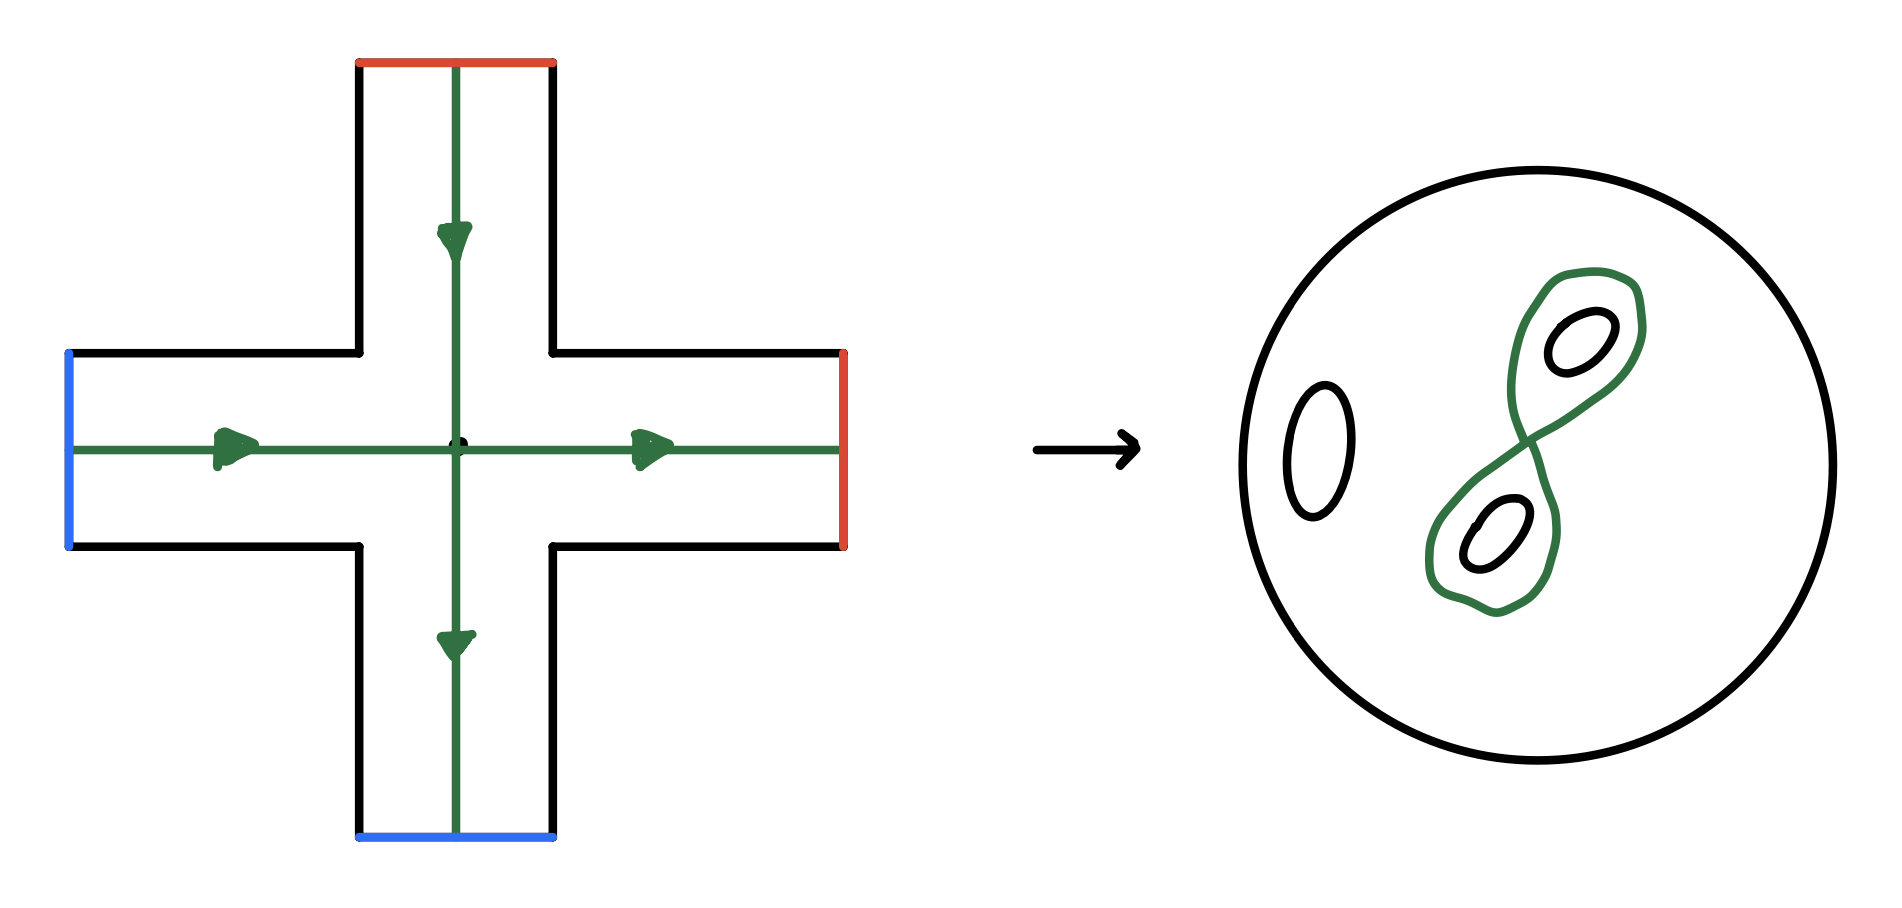
\includegraphics[scale=0.3]{problem10.png}
    \caption{A surface with self intersecting geodesics.}
  \end{figure}
  Since the attaching maps are affine, the flat connection on $\A^2$ descends to this quotient surface. Clearly, the path pictured in Figure~1 is a geodesic motion on this surface -- and an immersion of $S^1$ to a submanifold homeomorphic to $S^1\vee S^1$.
\end{solution}

\end{document}
